% 轨道参数 时间变量
% 轨道初值条件|轨道几何参数|轨道时间变量

\pentry{开普勒问题\upref{CelBd},开普勒第一定律的证明\upref{Keple1}}

在“开普勒第一定律的证明”中,我们得到了极坐标下的轨道方程
\begin{equation}\label{OribP_eq1} 
r=\frac{p}{1+e \cos\theta}
\end{equation}
其中,$p=L^2/(mk)$,$e=A/(mk)$.

对于轨迹上任意一点,容易求出质点在该处的速度矢量.可将速度矢量分解为切向速度 $v_\tau$ 与法向速度 $v_n$.在极坐标系中,切向速度可表示为 $v_\tau =r \dot\theta$,角动量为 $\bvec L  = mr^2\dot{\theta}\uvec z$,因此,切向速度为
\begin{equation}\label{OribP_eq2} 
v_\tau =\frac{L}{mr}
\end{equation}

另有法向速度 $v_n=\dot r$,对\autoref{OribP_eq1} 求导可得
\begin{equation} \label{OribP_eq3}
v_n =\dv{r}{t}=-\frac{ep\dot{\theta}\sin\theta}{(1+e\cos\theta)^2}=-\frac{epL\sin\theta}{mr^2(1+e\cos\theta)^2}=-\frac{A\sin\theta}{mL}
\end{equation}

\subsection{初值条件}
由轨道方程\autoref{OribP_eq1} 可知,轨道上 $\theta=0$ 的点距离坐标原点最近,并且由\autoref{OribP_eq2} 和 \autoref{OribP_eq3} 可以发现,该点处的切向速度最大,法向速度为零.在恒星-行星系统中,称这个最近点为“\bb{近日点}”,通常取该点的运动状态为初值条件.记这个最近距离为 $r_0$,该点处速度为 $v_0$.由此初值条件可得
\begin{align}
L &= mv_0r_0\\
A &= m^2v_0^2r_0-mk=m^2\qty(v_0^2r_0-GM)\\
e &= \frac{A}{mk}=\frac{v_0^2r_0}{GM}-1 
\end{align}

轨道上任意一点处,质点所具有的机械能为
\begin{equation} 
E =\frac{1}{2}m(v_{\tau}+v_n)^2-\frac{k}{r}
\end{equation}
由于系统不受外力或外力矩作用,故机械能守恒,由初值条件亦可求出系统机械能
\begin{equation} \label{OribP_eq8}
\begin{aligned}
E &=\frac{1}{2}mv_0^2-\frac{k}{r_0}\\
   &=\frac{L^2}{2mr_0^2}-\frac{k}{r_0}\\
   &=\frac{L^2}{2m}\frac{(1+e)^2)}{p^2}-\frac{k(1+e)}{p}\\
   &=\frac{mk^2}{2L^2}\qty(e^2-1)
\end{aligned}
\end{equation}
\autoref{OribP_eq8} 与“开普勒问题”中\autoref{CelBd_eq2} 所给出的轨道离心率与能量、角动量的关系式一致.

由此可见,初值条件可以唯一确定轨道的形状、大小等几何参数.

\subsection{时间变量}
在许多实际应用中,往往需要确定天体位置与时间的关系.比如常见的椭圆轨道,我们不仅需要知道周期,还需要计算天体运行至任意位置的时间.下面就对时间参数展开讨论.

可将极坐标下的角动量表达式 $ L  = mr^2\dot{\theta}$ 改写为
\begin{equation} 
\dv{\theta}{t}=\frac{L}{mr^2}
\end{equation}
将轨道方程\autoref{OribP_eq1} 代入,并分离变量
\begin{equation}
\dd{t}=\frac{L^3}{mk^2}\frac{\dd{\theta}}{(1+e\cos\theta)}
\end{equation}
方程两边积分,可得
\begin{equation}\label{OribP_eq11}
t-t_0 = \frac{L^3}{mk^2}\int_0^{\theta} \frac{\dd{\theta}}{(1+e\cos\theta)^2}
\end{equation}
其中 $t_0$ 为初始时间,习惯上取 $\theta=0$ 的时刻为时间的零点,即 $t_0=0$ .等号右边的积分根据轨道形状有不同的形式.

\subsubsection{圆轨道}
圆轨道是最简单的情况,离心率 $e=0$,可得
\begin{align}
t &=\frac{L^3}{mk^2}\theta \\
v^2r &=GM 
\end{align}
沿圆轨道运动的天体,角速度恒定,即\bb{匀速圆周运动}.令 $\theta=2\pi$ 可得运转周期为
\begin{equation}
T=\frac{2\pi L^3}{mk^2}=\frac{2\pi v^3r^3}{GM}=2\pi \sqrt{\frac{r^3}{GM}}
\end{equation}

\subsubsection{椭圆轨道}
椭圆轨道是最常见的情形,离心率 $0<e<1$
\begin{equation}\label{OribP_eq14}
t = \frac{L^3}{mk^2\qty(1-e^2)^{\frac{3}{2}}}\qty[2\arctan(\sqrt{\frac{1-e}{1+e}}\tan\frac{\theta}{2})-\frac{e\sqrt{1-e^2}\sin\theta}{1+e\cos\theta}]
\end{equation}
规定当 $(n-1)\pi<\theta \les n\pi$ 时,$\arctan(\sqrt{\frac{1-e}{1+e}}\tan\frac{\theta}{2})$ 在 $(\frac{n-1}{2}\pi,\frac{n}{2}\pi]$ 范围内取值.

同样的,令 $\theta=2\pi$ 可得运转周期为
\begin{equation}
T=\frac{2\pi L^3}{mk^2\qty(1-e^2)^{\frac{3}{2}}}
\end{equation}

根据\autoref{OribP_eq14}绘制的时间—角度变化规律,如\autoref{OribP_fig1} 所示
\begin{figure}[ht]
\centering
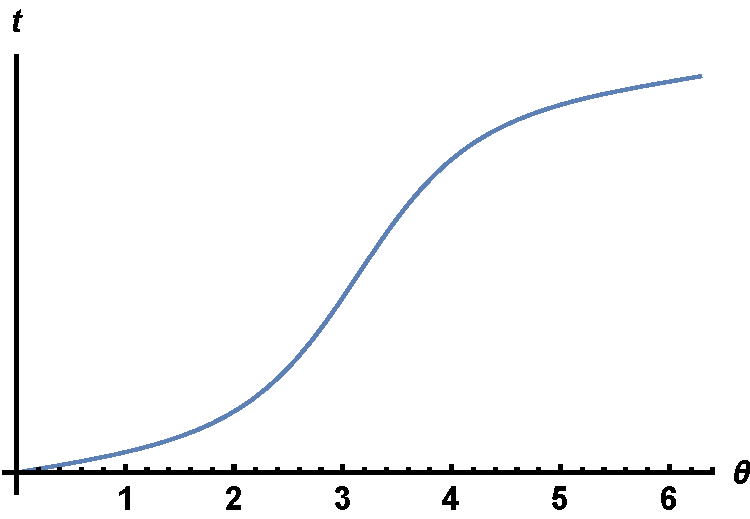
\includegraphics[width=6cm]{./figures/OribP1.pdf}
\caption{椭圆轨道时间变量} \label{OribP_fig1}
\end{figure}

\subsubsection{抛物线轨道}
抛物线轨道离心率 $e=1$
\begin{equation}
t = \frac{L^3}{2mk^2}\tan(\frac{\theta}{2})+\frac{1}{6}\tan[3](\frac{\theta}{2})
\end{equation}
在抛物线轨道上运动的天体,其动能与势能之和为\bb{零}.

\subsubsection{双曲线线轨道}
双曲线轨道离心率 $e>1$
\begin{equation}
t = \frac{L^3}{mk^2\qty(e^2-1)}\qty[\frac{e\sin\theta}{1+e\cos\theta}-\frac{1}{\sqrt{e^2-1}}\ln(\frac{\sqrt{e+1}+\sqrt{e-1}\tan\frac{\theta}{2}}{\sqrt{e+1}-\sqrt{e-1}\tan\frac{\theta}{2}})]
\end{equation}
双曲线轨道的时间—角度变化规律,如\autoref{OribP_fig2} 所示
\begin{figure}[ht]
\centering
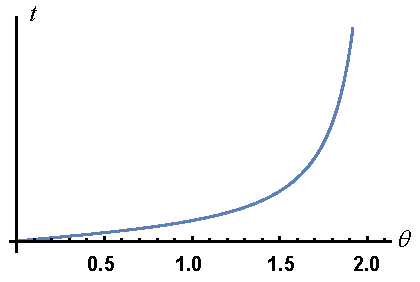
\includegraphics[width=6cm]{./figures/OribP2.pdf}
\caption{双曲线轨道时间变量} \label{OribP_fig2}
\end{figure}


由于\autoref{OribP_eq11} 中的被积函数在其有效定义域上为正值,因此所得的时间 $t$ 单调递增,即 $\theta$ 与 $t$ 存在一一对应的关系.然而位置—时间的关系式往往涉及超越方程的求解,不能用初等函数式表达,只能借助牛顿迭代法等数值方法计算.

